\subsection{Whitened Stochastic Variational Gaussian Processes}
\label{sec:variational_results}

As a first application, we demonstrate that the msMINRES-CIQ whitening procedure $\bK^{-1/2} \bb$ can increase the fidelity of {\bf stochastic variational Gaussian processes (SVGP)} \cite{hensman2013gaussian,hensman2015scalable,matthews2017scalable}.
These models are used for non-conjugate likelihoods (e.g.~binary classification) or for large datasets that do not fit into memory.
SVGP forms an approximate posterior
$
  p(f(\bx) \mid \bX, \by) \approx q(f(\bx)) = \Evover{q(\bu)}{ p\left( f(\bx) \mid \bu \right)},
$
where $\bu \in \reals^M$ are {inducing function values} (see \citep{hensman2015scalable,matthews2017scalable} for a detailed derivation).
$q \left( \bu \right)$ is a Gaussian variational distribution parameterized by mean $\bmm \in \reals^M$ and covariance $\bS \in \reals^{M \times M}$.
$\bmm$ and $\bS$ (as well as the model's kernel/likelihood hyperparameters) are chosen to maximize the variational ELBO:
%
\begin{align*}
  \loglik_\text{ELBO}\bigl\{ q(\bu) \! = \! \normaldist{\bmm}{\bS} \bigr\} &= \textstyle\sum_{i=1}^N \Evover{q(f(\bx^{(i)}))}{  \: \log p( y^{(i)} \mid f(\bx^{(i)}) ) } - \kl{ q(\bu) }{ p(\bu) }.
\end{align*}
%
Rather than directly learning $\bmm$ and $\bS$, it is more common to learn the \emph{whitened parameters} \cite{kuss2005assessing,matthews2017scalable}:
$$ \bmm' = \bK_{\bZ\bZ}^{- 1/ 2} \bmm, \quad \bS' = \bK_{\bZ\bZ}^{-1 / 2} \bS \bK_{\bZ\bZ}^{-1 / 2}. $$
Under these coordinates, the KL divergence term is
$\frac{1}{2} ( \bmm^{\prime \top} \bmm' + \tr{ \bS' } - \log \vert \bS' \vert - M ),$
%
which doesn't depend on $p(\bu)$ and therefore is relatively simple to optimize.
The posterior distribution $q(f(\bx)) = \normaldist{\ameantest{\bx}}{\avartest{\bx}}$ is given by
%
\begin{equation}
  \begin{split}
    \ameantest{\bx} &= \bk_{\bZ\bx}^\top \bK_{\bZ\bZ}^{-\frac 1 2} \bmm',
    \\
    \avartest{\bx} &= k(\bx, \bx) -
      \bk_{\bZ\bx}^\top \bK_{\bZ\bZ}^{-\frac 1 2} \left( \bI - \bS' \right) \bK_{\bZ\bZ}^{-\frac 1 2} \bk_{\bZ\bx}.
  \end{split}
  \label{eqn:approx_pred_dist}
\end{equation}

\paragraph{Time and space complexity.}
During training, we repeatedly compute the ELBO and its derivative, which requires computing \cref{eqn:approx_pred_dist} and its derivative for a minibatch of data points.
Optimization typically requires up to $10,\!000$ iterations of training \citep[e.g.][]{salimbeni2018natural}.
We note that $\bK_{\bZ\bZ}^{-1 / 2} \bb$ (and its derivative) is the most expensive numerical operation during each ELBO computation.
If we use Cholesky to compute this operation, the time complexity of SVGP training is $\bigo{M^3}$.
On the other hand, msMINRES-CIQ-based SVGP training is only $\bigo{J M^2}$, where $J$ is the number of msMINRES iterations.
Both methods require $\bigo{M^2}$ storage for the $\bmm'$ and $\bS'$ parameters.

\paragraph{Natural gradient descent with msMINRES-CIQ.}
The size of the variational parameters $\bmm'$ and $\bS'$ grows quadratically with $M$.
This poses a challenging optimization problem for standard gradient descent methods.
To adapt to the large $M$ regime, we rely on {\bf natural gradient descent (NGD)} to optimize $\bmm'$ and $\bS'$ \citep[e.g.][]{hensman2012fast,salimbeni2018natural}.
At a high level, these methods perform the updates $[\bmm, \:\: \bS] \gets [\bmm, \:\: \bS] - \varphi \: \bFS^{-1} \: \nabla \loglik_\text{ELBO}$,
where $\varphi$ is a step size, $\nabla \loglik_\text{ELBO}$ is the ELBO gradient, and $\bFS$ is the {Fisher information matrix} of the variational parameters.
%\citet{salimbeni2018natural} find that NGD updates on $\bmm'$ and $\bS'$ allow for faster optimization than single-order optimizers.
%
Na\"ively, each NGD step requires $\bigo{M^3}$ computations with $\bmm'$ and $\bS'$, which would dominate the cost of CIQ-based SVGP.
Fortunately, we can derive a natural gradient update that only relies on matrix solves with $\bS'$, which take $\bigo{J M^2}$ time using preconditioned conjugate gradients.
Therefore, using NGD incurs the same \emph{quadratic} asymptotic complexity as msMINRES-CIQ.
See \cref{app:ngd} for the $\bigo{M^2}$ NGD update equations.

\paragraph{Experimental details.}
We compare msMINRES-CIQ-SVGP against Cholesky-SVGP on 3 large-scale datasets: a GIS dataset ({\bf 3droad}, $D=2$), a monthly precipitation dataset ({\bf Precipitation}, $D=3$), and a tree cover dataset ({\bf Covtype}, $D=54$).
Each task has between $N=70,\!000$ and $N=500,\!000$ training data points.
For 3droad we use a Gaussian observation model.
The Precipitation dataset has noisier observations; therefore we apply a Student-T observation model.
Finally, we reduce the CovType dataset to a binary classification problem and apply a Bernoulli observation model.
We train models with $ 10^3 \le M \le 10^4$.
Each dataset is randomly split into $75\%$ training, $10\%$ validation, and $15\%$ testing sets; $\bx$ and $y$ values are scaled to be zero mean and unit variance.
All models use a constant mean and a Mat\'ern 5/2 kernel, with lengthscales initialized to $0.01$ and inducing points initialized by $K$-means clustering.
Each model is trained for $20$ epochs with a minibatch size of $256.$\footnote{
  The batch size is $512$ on the Covtype dataset due to its larger size.
}
We alternate between optimizing $\bmm'/\bS'$ and the other parameters, using NGD for the former and Adam \cite{kingma2014adam} for the latter.
Each optimizer uses an initial learning rate of $0.01$\footnote{
  On the Precipitation dataset, the initial learning rate is $0.005$ for NGD stability with the Student-T likelihood.
}, decayed by $10\times$ at epochs $1$, $5$, $10$, and $15$.
For CIQ we use $Q = 15$ quadrature points.
msMINRES terminates when the $\bc_j$ vectors achieve a relative norm of $0.001$ or after $J=200$ iterations.
Results are averaged over three trials.

The 3DRoad and CovType datasets are available from the UCI repository \citep{asuncion2007uci}.
For 3Droad, we only use the first two features---corresponding to latitude and longitude.
For CovType, we reduce the 7-way classification problem to a binary problem ($\mathtt{Cover\_Type} \in \{ 2, 3\}$ versus $\mathtt{Cover\_Type} \in \{ 0, 1, 4, 5, 6 \}$).
The Precipitation dataset is available from the IRI/LDEO Climate Data Library.\footnote{
  \url{http://iridl.ldeo.columbia.edu/maproom/Global/Precipitation/WASP_Indices.html}
}
This spatio-temporal dataset aims to predict the ``WASP'' index (Weighted Anomaly Standardized Precipitation) at various latitudes/longitudes.
Each data point corresponds to the WASP index for a given year (between 2010 and 2019)---which is the average of monthly WASP indices.
In total, there are 10 years and $10,\!127$ latitude/longitude coordinates, for a total dataset size of $101,\!270$.

\begin{figure}[t!]
  \centering
  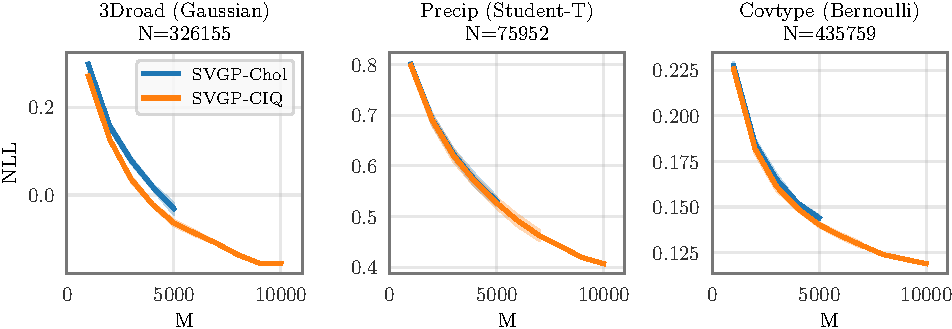
\includegraphics[width=\linewidth]{figures/variational_nll.pdf}
  \caption[Negative log likelihood (NLL) of Cholesky versus msMINRES-CIQ SVGP models.]{
    Negative log likelihood (NLL) of Cholesky versus msMINRES-CIQ SVGP models.
    {\bf Left:} 3DRoad dataset ($N=326155, D=2$, Gaussian likelihood).
    {\bf Middle:} Precipitation dataset ($N=75952, D=3$, Student-T likelihood).
    {\bf Right:} CoverType dataset ($N=435759, D=54$, Bernoulli likelihood).
    NLL improves with more inducing points ($M$), and Cholesky and msMINRES-CIQ models have similar performance.
    However msMINRES-CIQ models train faster than their Cholesky counterparts.
  }
  \label{fig:variational_nll}
\end{figure}

\begin{figure}[t!]
  \centering
  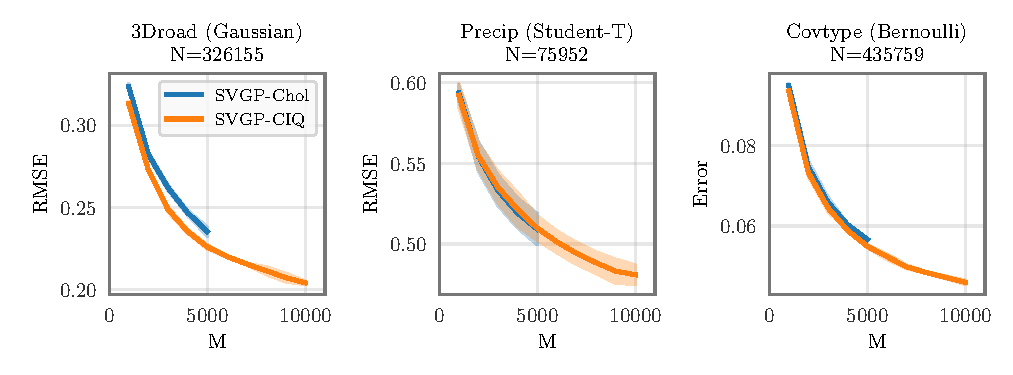
\includegraphics[width=\linewidth]{figures/variational_error.pdf}
  \caption[Error of Cholesky versus msMINRES-CIQ SVGP models.]{
    Error of Cholesky versus msMINRES-CIQ SVGP models.
    {\bf Left:} 3DRoad dataset RMSE ($N=326155, D=2$, Gaussian likelihood).
    {\bf Middle:} Precipitation dataset RMSE ($N=75952, D=3$, Student-T likelihood).
    {\bf Right:} CoverType dataset $0/1$ error ($N=435759, D=54$, Bernoulli likelihood).
  }
  \label{fig:variational_error}
\end{figure}

\paragraph{Results.}
The two methods achieve very similar test-set negative log likelihood (\cref{fig:variational_nll}) and RMSE (\cref{fig:variational_error}).
We note that there are small
differences in the optimization dynamics, which is to be expected since $\bK_{\bZ\bZ}^{-1/2} \bk_{\bZ\bx}$ can differ by an orthogonal
transformation when computed with msMINRES-CIQ versus Cholesky.
The key difference is the training time:
with $M=5,\!000$ inducing points, msMINRES-CIQ models are up to \emph{5.6x faster} than Cholesky models (on a Titan RTX GPU).
Moreover, msMINRES-CIQ models with $M=8,\!000$-$10,\!000$ take roughly the same amount of time as $M=5,\!000$ Cholesky models.
Note we do not train $M > 5,\!000$ Cholesky models as doing so would require $2$-$10$ days.

\begin{figure}[t!]
  \centering
  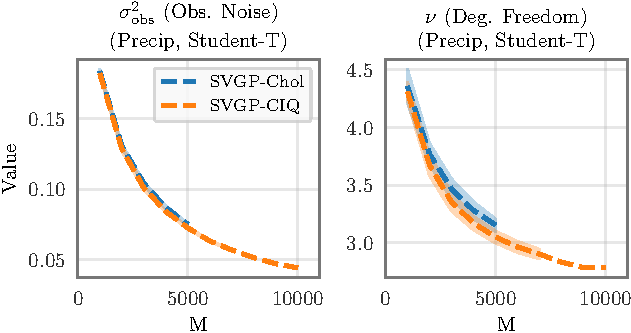
\includegraphics[width=\linewidth]{figures/variational_stats.pdf}
  \caption[Hyperparameters of Cholesky and CIQ SVGP models.]{
    Hyperparameters as a function of inducing points ($M$) for Chol-SVGP and msMINRES-CIQ-SVGP (Precipitation dataset, Student-T likelihood).
    As $M$ increases, the kernel outputscale (left) also increases.
    At the same time, the estimated observational noise (middle) decreases as does the estimated degrees of freedom (right), reflecting a heavier-tailed noise distribution.
    This suggests that, with larger $M$, SVGP models can find more signal in the data.
  }
  \label{fig:variational_stats}
\end{figure}

\paragraph{Effects of increased inducing points.}
We find that accuracy improves with increased $M$ on all datasets.
Scaling from $M=5,\!000$ to $M=10,\!000$ reduces test-set NLL by $0.1$ nats on the 3droad and Precipitation datasets.
We find similar reductions in predictive error.
By scaling more readily to large $M$, msMINRES-CIQ enables high-fidelity variational approximations that would be computationally prohibitive with Cholesky.
We also find that increasing $M$ changes the values of the learned kernel/likelihood hyperparameters.
In \cref{fig:variational_stats} we plot the learned hyperparameters of the Precipitation SVGP models:
%
\begin{enumerate*}
  \item $o^2$ (the kernel outputscale)---which roughly corresponds to variance explained as ``signal'' in the data;
  \item $\sigma^2_\text{obs}$---which roughly corresponds to variance explained away as observational noise; and
  \item $\nu$ (degrees of freedom)---which controls the tails of the noise model (lower $\nu$ corresponds to heavier tails).
\end{enumerate*}
%
As $M$ increases, we find that the observational noise parameter decreases by a factor of $4$---down from $0.19$ to $0.05$---while the $\nu$ parameter also decreases.
Models with larger $M$ values can more closely approximate the true posterior \cite{hensman2013gaussian}; therefore, we expect that the larger-$M$ likelihoods more closely correspond to the true parameters.
This confirms findings from \citet{bauer2016understanding}, who argue that variational approximations with small $M$ tend to overestimate the amount of noise in datasets.
